\documentclass{article}
\usepackage{graphicx}
\usepackage[margin=1in]{geometry}
\usepackage{hyperref}
\usepackage{setspace}
\usepackage[T1]{fontenc}
\usepackage{lmodern}
\usepackage{tikz}
\usepackage{apacite}
\bibliographystyle{apacite}
\usetikzlibrary{positioning,arrows.meta,fit,calc,shadows.blur}
\doublespacing

\title{CSC 487 Final Project Report}
\author{Ahad Jiva, Pranav Nallaperumal, Pranav Krishna, Milad Chabok}
\date{March 17th, 2026}

\begin{document}

\maketitle

\section{Introduction}

We implemented a Binary classifier to tackle the problem of identifying fraudulent credit card transactions. We used a dataset containing 1.3 million different transactions and their associated data. The challenge we faced was a severe class imbalance: fraudulent transactions do not occur as often as legitimate ones. In our dataset, only 0.58\% of the transactions were fraudulent. We tried several approaches to solve this problem, including minority class oversampling, different weighted loss functions, and various encoding strategies for the categorical features.

\section{Background}

Credit card fraud detection has progressed from classic statistical detection to machine learning and modern deep learning methods. Early work used logistic/probabilistic methods(e.g., risk scoring and unsupervised anomaly detection frameworks). They also cemented extreme class imbalance and ever-changing fraudulent behavior as core challenges. Tree and Margin-based methods came to be used more to model nonlinear interactions in tabular data as transaction scale increased (e.g. Decision trees, SVMs and Random forests).

Class imbalance has been a persistent issue across these generations of methods: fraud transactions are rare, so accuracy alone would be a misleading metric/statistic. Prior work emphasises resampling, and cost-sensitive approaches (including SMOTE, its variants, and weighted loss functions) alongside recall/precision/F1 based evaluations. More recent work applies Neural and Sequence Models like LSTMs to capture temporal spending behavior and adapt to concept drift.

Based on the above track record, we evaluated a deep tabular dataset with features we engineered, loss function choices for the imbalance problem, and oversampling techniques we evaluated on non-accuracy metrics as described below.


\section{Data}

Our dataset contains a mix of numerical and categorical features for each transaction, including transaction amount, purchase category, timestamp, etc. In total, it includes about 1.3 million transactions, with a severe class imbalance, where only about 0.58\% are labeled fraudulent (is\_fraud = 1). Numerical fields (e.g. amount, latitude/longitude, city population, Unix time) capture transaction scale and location patterns, while categorical fields (e.g. merchant category, state, gender, cardholder occupation) provide behavioral context. We excluded the credit card number and transaction UUID fields from modeling since they are essentially unique and have no bearing on transaction risk. Instead, we focused on generalizable fraud patterns.

\begin{center}
    \includegraphics*[width=\textwidth]{heatmap.png}
\end{center}

This heatmap tells us that fraud-risk is highly time-dependent. Rates almost bottom out during daytime/business hours and spike sharply late at night, with the most pronounced spikes around hours 22-23 across nearly all days. This pattern shows late transactions are disproportionately risky, while weekday differences are smaller than the hour-of-day effect.

\begin{center}
    \includegraphics*[width=\textwidth]{volume.png}
\end{center}

Transaction volume is relatively stable month-to-month with one clear surge around late 2019, while fraud rate fluctuates more sharply across months. This suggests temporal drift in fraud behavior: risk changes over time and is not simply proportional to transaction volume.

\section{Evaluation}

We first ran a baseline test with a simple model and no fancy data transformations to get baseline precision, recall, and F1 metrics. We also plotted Precision-Recall Curves and calculated Area Under the Curve for each model. With every technique that we implemented and tested, we compared these metrics to the baseline model to see which ones (or which combinations) improved our base performance the most.

\section{Methods and Results}

Our solution uses a feedforward MLP to classify transactions as either legitimate or fraudulent. The dataset contains a mix of numerical and categorical features for each transaction, including transaction amount, purchase category, timestamp, etc.

\begin{figure}[h]
\centering
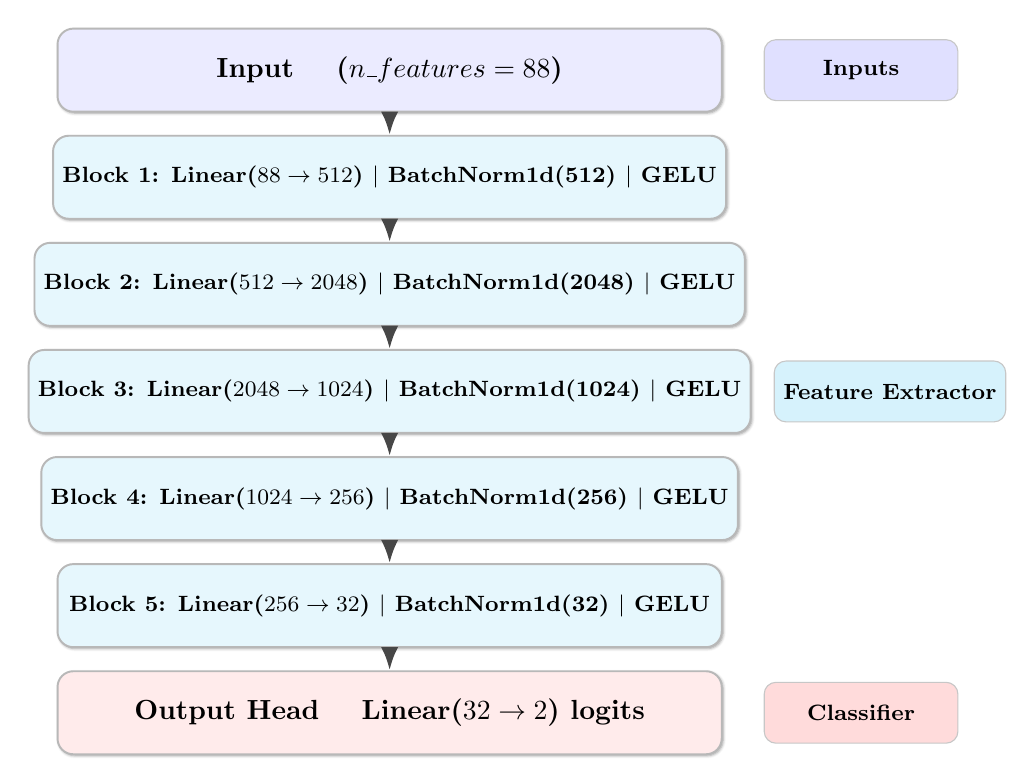
\begin{tikzpicture}[
    font=\sffamily,
    >=Latex,
    node distance=8pt,
    flow/.style={->, line width=1.2pt, draw=black!72},
    card/.style={
        draw=black!28,
        rounded corners=2mm,
        align=center,
        minimum width=240pt,
        minimum height=30pt,
        line width=0.7pt,
        blur shadow={shadow xshift=0.5pt, shadow yshift=-0.5pt, shadow blur radius=1pt}
    },
    inputcard/.style={card, fill=blue!8},
    hiddencard/.style={card, fill=cyan!10},
    outputcard/.style={card, fill=red!8},
    sidepill/.style={
        draw=black!22,
        rounded corners=1.5mm,
        fill=white,
        minimum width=70pt,
        minimum height=22pt,
        font=\bfseries\fontsize{8}{10}\selectfont
    }
]

\node[inputcard, font=\bfseries\fontsize{10}{12}\selectfont] (input) at (0,0) {Input \quad ($n\_features = 88$)};
\node[hiddencard, below=of input, font=\bfseries\fontsize{8}{10}\selectfont] (b1) {Block 1: Linear($88 \rightarrow 512$) $|$ BatchNorm1d(512) $|$ GELU};
\node[hiddencard, below=of b1, font=\bfseries\fontsize{8}{10}\selectfont] (b2) {Block 2: Linear($512 \rightarrow 2048$) $|$ BatchNorm1d(2048) $|$ GELU};
\node[hiddencard, below=of b2, font=\bfseries\fontsize{8}{10}\selectfont] (b3) {Block 3: Linear($2048 \rightarrow 1024$) $|$ BatchNorm1d(1024) $|$ GELU};
\node[hiddencard, below=of b3, font=\bfseries\fontsize{8}{10}\selectfont] (b4) {Block 4: Linear($1024 \rightarrow 256$) $|$ BatchNorm1d(256) $|$ GELU};
\node[hiddencard, below=of b4, font=\bfseries\fontsize{8}{10}\selectfont] (b5) {Block 5: Linear($256 \rightarrow 32$) $|$ BatchNorm1d(32) $|$ GELU};
\node[outputcard, below=of b5, font=\bfseries\fontsize{10}{12}\selectfont] (out) {Output Head \quad Linear($32 \rightarrow 2$) logits};

\draw[flow] (input) -- (b1);
\draw[flow] (b1) -- (b2);
\draw[flow] (b2) -- (b3);
\draw[flow] (b3) -- (b4);
\draw[flow] (b4) -- (b5);
\draw[flow] (b5) -- (out);

\node[sidepill, fill=blue!12] at ($(input.east)+(50pt,0)$) {Inputs};
\node[sidepill, fill=cyan!16] at ($(b3.east)+(50pt,0)$) {Feature Extractor};
\node[sidepill, fill=red!14] at ($(out.east)+(50pt,0)$) {Classifier};
\end{tikzpicture}
\caption{MLP architecture for fraud detection.}
\end{figure}

\subsection{Baseline Model}

To start, we only took the numerical data from the dataset and used that to train the model. We did not use any special techniques to account for the class imbalance; this experiment was to get a baseline performance reading from which we could measure our model's improvement.

\begin{table*}[h]
    \centering
    \begin{tabular}{|c|c|c|}
        \hline
        \textbf{Metric} & \textbf{Value} & \textbf{Improvement Over Baseline} \\
        \hline \hline
        Precision & 55.46\% & - \\
        \hline
        Recall & 27.49\% & - \\
        \hline
        F1 & 36.76\% & - \\
        \hline
    \end{tabular}
\end{table*}

\begin{center}
    \includegraphics*[width=0.75\textwidth]{base.png}
\end{center}

\subsection{LLM-Defined Job Categories}

The first categorical feature that we wanted to include was the cardholder's job; we felt that it would be a significant indicator of the existence of fraud. However, the dataset contained 494 possible values for the job feature, and applying one-hot encoding would have blown up our input vector and encountered the curse of dimensionality. Instead, we chose to feed the job categories into an LLM (specifically Gemini 3 Flash Preview), which analyzed the job categories and condensed them down into 10 broader categories. We then mapped each job to its broader category amongst these ten, and then applied one-hot encoding. With this technique, we improved recall with no effect on precision.

\begin{table*}[h]
    \centering
    \begin{tabular}{|c|c|c|}
        \hline
        \textbf{Metric} & \textbf{Value} & \textbf{Improvement Over Baseline} \\
        \hline \hline
        Precision & 55.66\% & 0.20\% \\
        \hline
        Recall & 30.87\% & 3.38\% \\
        \hline
        F1 & 39.71\% & 2.95\% \\
        \hline
    \end{tabular}
\end{table*}

\begin{center}
    \includegraphics*[width=0.75\textwidth]{llm.png}
\end{center}

\subsection{Minority Class Oversampling}

The next approach was to implement minority class oversampling. We implemented this by using the ImbalancedDatasetSampler sampler from the torchsampler library and passing it to the train set DataLoader. This forces the DataLoader to pick from the minority class at a higher rate, increasing the chance that the minority class appears in the training data. This had a significant impact on the model's performance.

\begin{table*}[h]
    \centering
    \begin{tabular}{|c|c|c|}
        \hline
        \textbf{Metric} & \textbf{Value} & \textbf{Improvement Over Baseline} \\
        \hline \hline
        Precision & 17.45\% & -38.01\% \\
        \hline
        Recall & 78.94\% & 51.45\% \\
        \hline
        F1 & 28.58\% & -8.18\% \\
        \hline
    \end{tabular}
\end{table*}

\begin{center}
    \includegraphics*[width=0.75\textwidth]{mco.png}
\end{center}

\subsection{SVMSMOTE}

Similar to the previous technique, we also tried using SVMSMOTE, which actually generates augmented data from the minority class and adds it to the train set. SVMSMOTE is a variant of SMOTE that uses an SVM algorithm to detect samples to use for generating synthetic samples. Notably, the SVMSMOTE technique did not improve over the baseline model as much as the ImbalancedDatasetSampler did, though the improvement is still significant. SVMSMOTE also took much longer to train, as the data augmentation process is computationally expensive.

\begin{table*}[h]
    \centering
    \begin{tabular}{|c|c|c|}
        \hline
        \textbf{Metric} & \textbf{Value} & \textbf{Improvement Over Baseline} \\
        \hline \hline
        Precision & 13.84\% & -41.62\% \\
        \hline
        Recall & 83.11\% & 55.62\% \\
        \hline
        F1 & 23.73\% & -13.03\% \\
        \hline
    \end{tabular}
\end{table*}

\begin{center}
    \includegraphics*[width=0.75\textwidth]{smote.png}
\end{center}

\subsection{One-Hot Encoding}

Our next strategy was to integrate the other categorical features into the input vector. We chose to leave out the credit card numbers and transaction UUID from all experiments, as they would not have provided much insight to the model. One-hot encoding was applied to gender, transaction category, and state. We used the transaction date and the cardholder's date of birth to calculate the age of the person making the transaction. In total, we increased the number of features of our input vector from 11 to 88. This provided the largest increase in model performance yet, outperforming both IDS and SVMSMOTE.

\begin{table*}[h]
    \centering
    \begin{tabular}{|c|c|c|}
        \hline
        \textbf{Metric} & \textbf{Value} & \textbf{Improvement Over Baseline} \\
        \hline \hline
        Precision & 44.94\% & -10.52\% \\
        \hline
        Recall & 85.86\% & 58.37\% \\
        \hline
        F1 & 59.00\% & 22.24\% \\
        \hline
    \end{tabular}
\end{table*}

\begin{center}
    \includegraphics*[width=0.75\textwidth]{ohe.png}
\end{center}

\subsection{Weighted MultiMargin Loss}

We now turn our attention to the loss function. Up until now, we used the default Cross-Entropy Loss function for training, but this function is blind to class imbalances. Our first experiment was to use a weighted Multi Margin loss function, where the weights were determined by the inverse frequency of the fraud and legitimate classes. Without SVMSMOTE and IDS but with one-hot encoding, this technique gave us the best result so far. Notably, MultiMargin loss does not have an MPS implementation, so training had to be performed on CPU.

\begin{table*}[h]
    \centering
    \begin{tabular}{|c|c|c|}
        \hline
        \textbf{Metric} & \textbf{Value} & \textbf{Improvement Over Baseline} \\
        \hline \hline
        Precision & 10.72\% & -44.74\% \\
        \hline
        Recall & 93.00\% & 65.51\% \\
        \hline
        F1 & 19.23\% & -17.53\% \\
        \hline
    \end{tabular}
\end{table*}

\begin{center}
    \includegraphics*[width=0.75\textwidth]{mml.png}
\end{center}

\subsection{Weighted CrossEntropy Loss}

Another weighted loss function we used was Cross-Entropy Loss. We used the same inverse-frequency derived weights as before, but with Cross Entropy instead. The improvement over Multi Margin loss was almost imperceptible, but because of its MPS implementation in torch, training was much faster. This loss function, along with one-hot encoding of categorical variables and the omission of SVMSMOTE and IDS, resulted in the best model performance overall.

\begin{table*}[h]
    \centering
    \begin{tabular}{|c|c|c|}
        \hline
        \textbf{Metric} & \textbf{Value} & \textbf{Improvement Over Baseline} \\
        \hline \hline
        Precision & 11.06\% & -44.40\% \\
        \hline
        Recall & 93.09\% & 65.60\% \\
        \hline
        F1 & 19.77\% & -16.99\% \\
        \hline
    \end{tabular}
\end{table*}

\begin{center}
    \includegraphics*[width=0.75\textwidth]{cel.png}
\end{center}

\section{Outlook}

Earlier in the quarter, we expected that handling the extreme class imbalance problem would be the dominant factor in performance and that oversampling techniques like SMOTE and its variants would provide the largest gains. We also expected adding categorical context/encodings (job, state, merchant category, gender) would help, but initially assumed the performance increase from these would be second to the earlier imbalance methods.
Our final results only partially matched those expectations. Imbalance-aware methods like weighted loss in combination with feature engineering and encodings made the biggest, most consistent improvements on our evaluation metrics. Oversampling often improved recall but introduced many false positives, hurting precision.

The main lesson is that for fraud detection, accuracy is misleading; precision/recall/F1 and tradeoff-aware evaluation are more meaningful. We also learned that data representation mattered more than making the MLP deeper.

If we continued, we would focus on: (1) threshold tuning and probability calibration, (2) time-based validation to handle concept drift, and (3) comparing against strong tabular baselines (e.g., XGBoost/LightGBM) plus richer temporal/geospatial features. Overall, we met our core goal by building a substantially improved fraud detector and identifying which techniques provide the highest return.

\nocite{*}
\bibliography{mybib.bib}

\end{document}